\documentclass[border=10pt]{standalone}

\usepackage{tikz}
\usepackage{tikzsymbols}
\usetikzlibrary{calc,patterns,shapes.geometric}

\def\centerarc[#1](#2)(#3:#4:#5){\draw[#1] ($(#2)+({#5*cos(#3)},{#5*sin(#3)})$) arc (#3:#4:#5);}

\begin{document}
	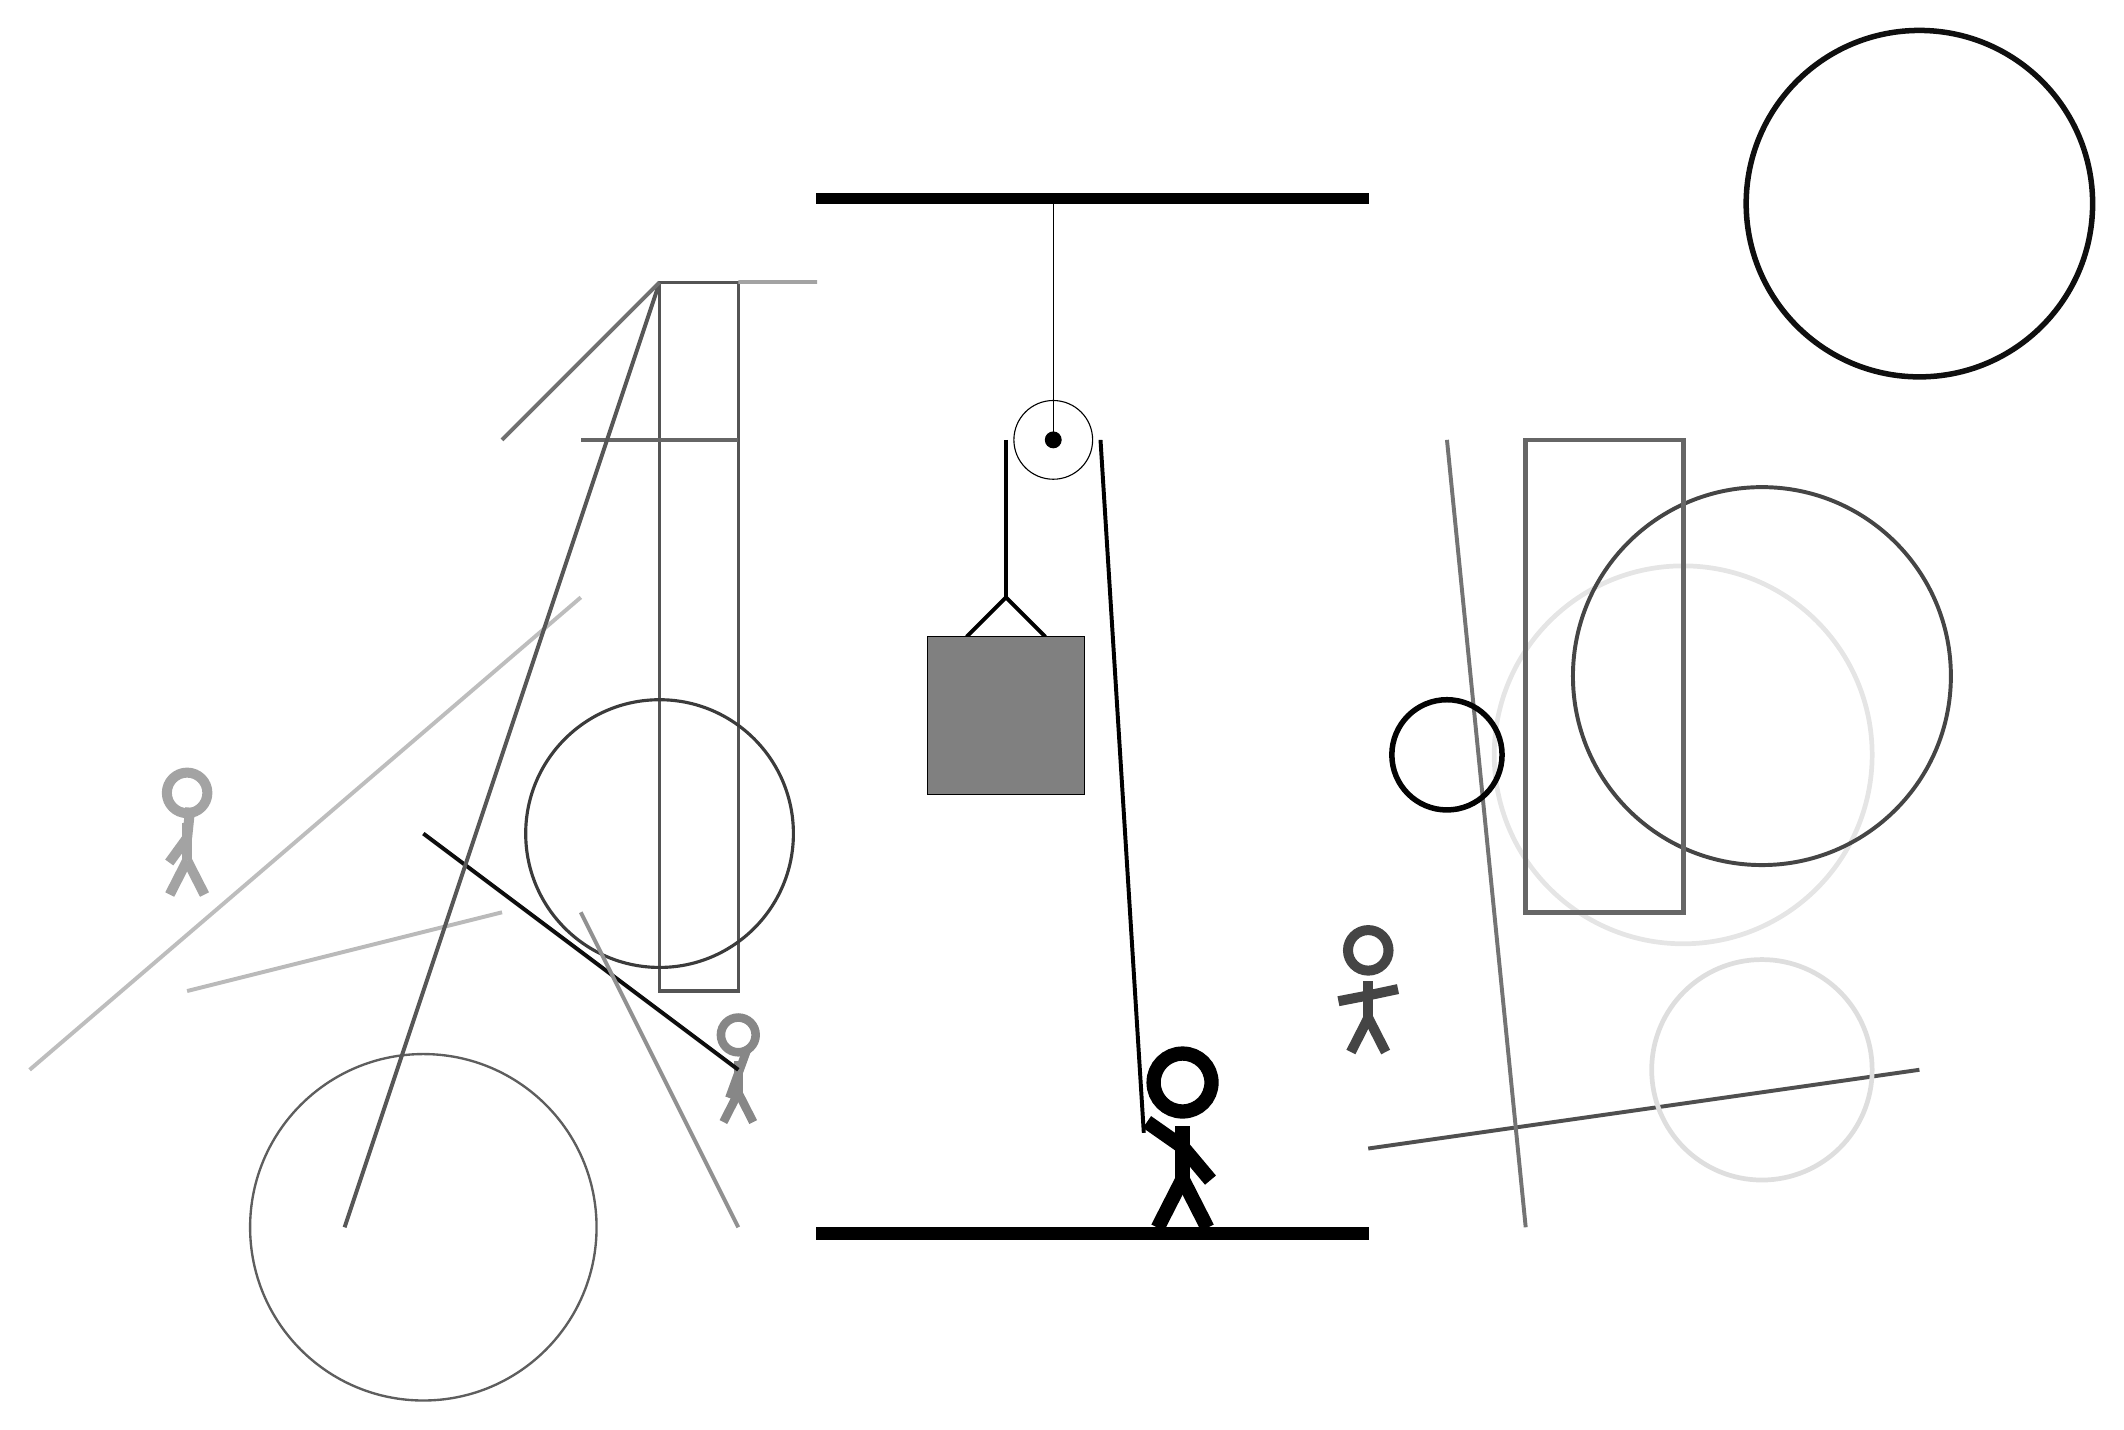
\begin{tikzpicture}
		%%%%% START %%%%%
		
		\draw[fill=black] (-2, 10) rectangle (5, 10.125);
		
		\draw (1, 7) circle (0.5);
		\draw[fill=black] (1, 7) circle (0.1);
		\draw (1, 10) -- (1, 7);
		
		\draw[line width=0.5mm] (-0.1, 4.5) -- (0.4, 5.0) -- (0.9, 4.5);
		\draw[fill=black!50] (-0.6, 4.5) rectangle (1.4, 2.5);
		
		\draw[line width=0.5mm] (0.4, 7) -- (0.4, 5.0);
		\centerarc[line width=0.5mm](1, 7)(0:180:0.6);
		\draw[line width=0.5mm](1.6, 7) -- (2.15, -1.8);
		
		\node at (2.6, -1.9) {\Strichmaxerl[10][-35][-50]};
		
		\node[line width=0.3mm, color=black!73] at (5, 0) {\Strichmaxerl[7][11][12]};
		
		\draw[line width=0.5mm, color=black!26](-5, 5) -- (-12, -1);
		\draw[line width=0.5mm, color=black!69](5, -2) -- (12, -1);
		\node[line width=0.3mm, color=black!36] at (-10, 2) {\Strichmaxerl[7][54][84]};
		\node[line width=0.3mm, color=black!47] at (-3, -1) {\Strichmaxerl[6][70][70]};
		\draw[line width=0.5mm, color=black!27](-6, 1) -- (-10, 0);
		
		\draw[line width=0.5mm, color=black!95](-3, -1) -- (-7, 2);
		\draw[line width=0.4mm, color=black!67] (-4, 9) rectangle (-3, 0);
		\draw [line width=0.6mm, color=black!10](9, 3) circle (2.4);
		\draw[line width=0.5mm, color=black!55](6, 7) -- (7, -3);
		\draw [line width=0.4mm, color=black!77](-4, 2) circle (1.7);
		
		\draw [line width=0.6mm, color=black!13](10, -1) circle (1.4);
		\draw [line width=0.3mm, color=black!63](-7, -3) circle (2.2);
		
		\draw[line width=0.5mm, color=black!60](-3, 7) -- (-5, 7);
		\draw[line width=0.5mm, color=black!43](-5, 1) -- (-3, -3);
		\draw [line width=0.7mm, color=black!99](6, 3) circle (0.7);
		\draw[line width=0.5mm, color=black!66](-4, 9) -- (-8, -3);
		\draw [line width=0.5mm, color=black!73](10, 4) circle (2.4);
		\draw[line width=0.5mm, color=black!56](-6, 7) -- (-4, 9);
		\draw[line width=0.6mm, color=black!60] (7, 7) rectangle (9, 1);
		\draw[line width=0.5mm, color=black!36] (-2, 9) rectangle (-3, 9);
		\draw [line width=0.7mm, color=black!94](12, 10) circle (2.2);
		
		
		\draw[fill=black] (-2, -3) rectangle (5, -3.15);
		
		%%%%% END %%%%%
	\end{tikzpicture}
\end{document}